%Estad\'istica Descriptiva: Correlaci\'on y Regresi\'on Lineal
\begin{itemize}
	\item Objetivo: Obtener informaci\'on desde una muestra, que permita entender o formular hip\'otesis acerca del fen\'omeno que se estudia.
	\item Tipos de An\'alisis
	\begin{itemize}
		\item Describir c\'omo se comporta una variable
		\item Describir c\'omo una variable afecta el comportamiento de a otra
		\item Describir c\'omo interaccionan varias variables
	\end{itemize}
	\subsection{An\'alisis Bivariado}
		\subsubsection{Correlaci\'on}
		Medida cuantitativa del grado de asociaci\'on entre dos variables X e Y continuas
		\begin{itemize}
			\item Covarianza: Medici\'on de los cambios con respecto al nivel medio de cada variable.\\
					 La medida depende de las magnitudes absolutas de x e y, por lo que una mayor covarianza no significa mayor asociaci\'on.\\
					 $$ cov(x,y)\ =\ \frac{1}{n}\sum_{i=1}^{n}\ (x_i\ -\ \bar{x})(y_i\ -\ \bar{y}) $$
			\item Coeficiente de Correlaci\'on de Pearson: Normaliza la covarianza con una medida de dispersi\'on para X y para Y. Es acotada entre -1 y 1.
					 $$\rho_{xy}\ =\ \frac{cov(x,y)}{\sigma_x\sigma_y}$$


			\begin{itemize}
				\item Observaciones
				\begin{itemize}
					\item Si x e y tienen una relaci\'on lineal exacta, la correlaci\'on de Pearson es igual al signo de la pendiente.
					\item $cov(x,y)\ =\ a\cdot var(x)$ 
					\item $var(y)=\ a^2\cdot var(x)$ 
					\item Una correlaci\'on nula indica que no hay relaci\'on aparente entre las variables (penditene 0). 
				\end{itemize}
				\item Correlaci\'on y Ruido\\
					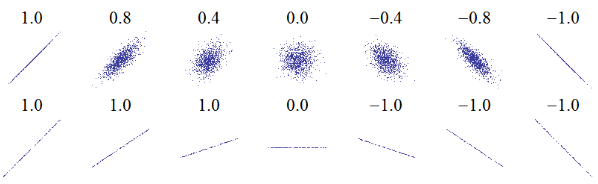
\includegraphics[height=3.5cm]{images/ruido}
				\item Limitaciones: Para un mismo valor del coeficiente pearson...\\
					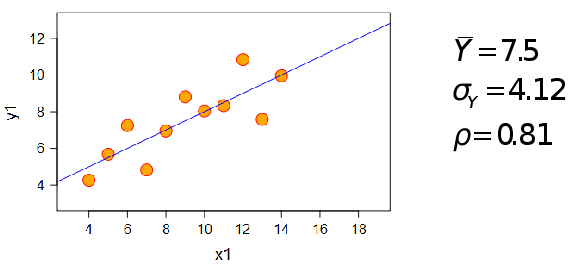
\includegraphics[height=3.5cm]{images/cap4-limit_pearson1.png}\\
					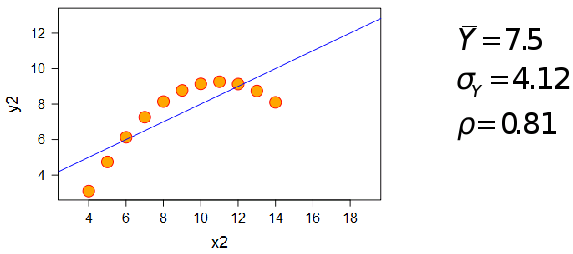
\includegraphics[height=3.5cm]{images/cap4-limit_pearson2.png}\\
					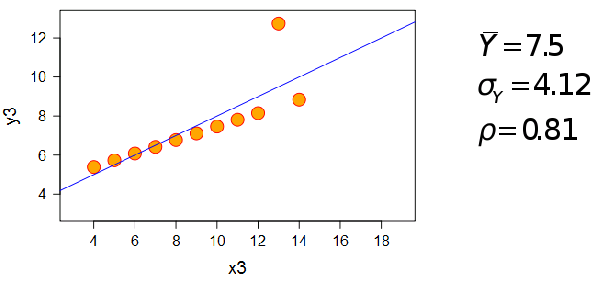
\includegraphics[height=3.5cm]{images/cap4-limit_pearson3.png}\\
					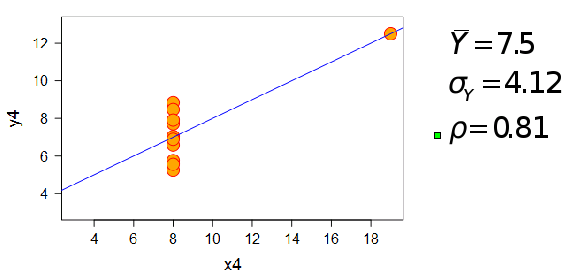
\includegraphics[height=3.5cm]{images/cap4-limit_pearson4.png}
			\end{itemize}
		\end{itemize}
		\subsubsection{Regresi\'on}
			Modelo de una variable y (dependiente) como funci\'on de otra x (independiente).\\
			$$Y\ =\ f(X)+\varepsilon$$
		\begin{itemize}
			\item Regresi\'on Lineal: Ajustar el modelo lineal consiste en buscar par\'ametros b0 y b1 que hagan el modelo adecuado.
				$$f(x)\ =\ b_1x\ +\ b_0$$
			\begin{itemize}
				\item Estimando los coeficientes: Minimizar error cuadr\'atico\\
					$$I^2(x,y)\ =\ (y-f(x))^2$$
					$$I^2(x,y)\ =\ (y-b_1x-b_0)^2\ = \varepsilon^2$$\\
					Ahora buscamos minimizar el error promedio:\\
					$$R_s\ =\ \sum_{x_i\ \epsilon\ S}(y_i-b_1x_i-b_0)^2$$
					$$R_s\ =\ \sum_{x_i\ \epsilon\ S}I^2(x_i,y_i)$$
					Y despues de analizar las derivadas en funci\'on de $b_0$, $b_1$ y ver unos cuantos determinantes..
					$$b_1\ =\ \frac{cov(x,y)}{var(x)}$$
					$$b_0\ =\ \bar{y}\ -\ \frac{cov(x,y)}{var(x)}\bar{x}$$
				\item An\'alisis de la Varianza: Sirve para ver que tan bueno es nuestro modelo descriptivo.\\
				\begin{itemize}
					\item Variabilidad explicada por el modelo: $$S(\hat{y})\ =\ \sum_{i}(\hat{y_i}\ -\ \bar{\hat{y_i}})^2\ =\ \sum_{i}(\hat{y_i}\ -\ \bar{y_i})^2$$
					\item Variabilidad NO explicada por el modelo:$$R_S\ =\ \sum_{i}\varepsilon_{i}^{2}\ =\ \sum_{i}(y_i\ -\ \hat{y})^2$$
					\item Variabilidad Total de Y:
								$$S(y)\ =\ \sum_{i}(y_i\ -\ \bar{y})^2$$\\
								Y esto es igual a la variabilidad explicada + la no explicada:
								$$S(y)\ =\ \sum_{i}(\hat{y_i}\ -\ \bar{y_i})^2\ +\ \sum_{i}(y_i\ -\ \hat{y})^2 $$
				\end{itemize}
				\item Coeficiente de Determinaci\'on: Fracci\'on de la variabilidad que s\'i es explicada por el modelo lineal (\% de ajuste):
					$$D\ =\ \frac{S(\hat{y})}{S(y)}$$\\
					Y ahora si sabemos que:
					$$S(\hat{y})\ =\ \sum_{i}(\hat{y_i}-\bar{\hat{y_i}})^2\ =\ \sum_{i}(\hat{b_0}\ +\ \hat{b_1}x_i \ -\ \bar{y})^2$$
					$$S(\hat{y})\ =\ \sum_{i}(\ \hat{b_1}x_i \ +\ \hat{b_1}\bar{x})^2$$
					$$S(\hat{y})\ =\ \hat{b_1^2}\cdot n\cdot var(x)$$\\
					El coeficiente nos queda:
					$$D\ =\ \frac{\hat{b_1^2)}\cdot n\cdot var(x)}{n\cdot var(y)}$$
					$$D\ =\ \frac{\hat{b_1^2)}\cdot var(x)}{var(y)}$$\\
					Y por \'ultimo, reemplazando el b:
					$$D\ =\ \rho_{xy}^2$$
					$$\therefore\ D\ =\ \frac{cov^2(x,y)}{var(x)\ var(y)}$$
			\end{itemize}
			\item Regresiones con trasnformaci\'ones lineales: Uno construye un modelo lineal en una variable independiente auxiliar.
				$$Y\ =\ b_0\ +\ b_1ln(X)\ +\ \varepsilon$$
				$$Z\ =\ X^2$$
	\end{itemize}
\end{itemize}
